\section{Work Breakdown Structure}
\label{dsePPWBS}
The work breakdown can be seen in figures \ref{wbspp}, \ref{wbsbr}, \ref{wbsmtr} and \ref{wbsfr} on pages \pageref{wbspp} to \pageref{wbsfr}. Just like with the workflow diagrams, the WBS was broken down into four logical parts. The Gantt chart in section \ref{dsePPTimeline} displays a more detailed look at the tasks. The two can be thought of as complementary tool.

%\newpage
\begin{figure} [H]
\begin{center}
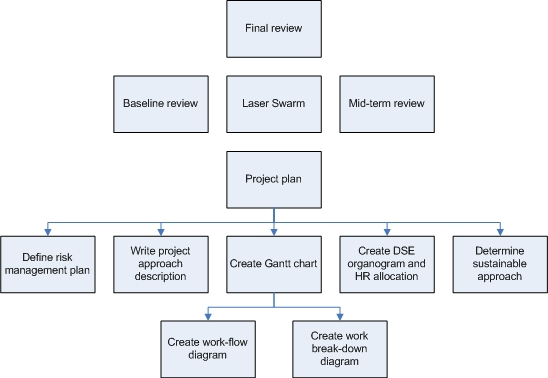
\includegraphics[width=1.0\textwidth, angle=0]{chapters/img/Work_break_down_structure_PP.jpg}
\end{center}
\caption{Work breakdown structure leading to PP.}
\label{wbspp}
\end{figure}
%\newpage
\begin{figure} [H]
\begin{center}
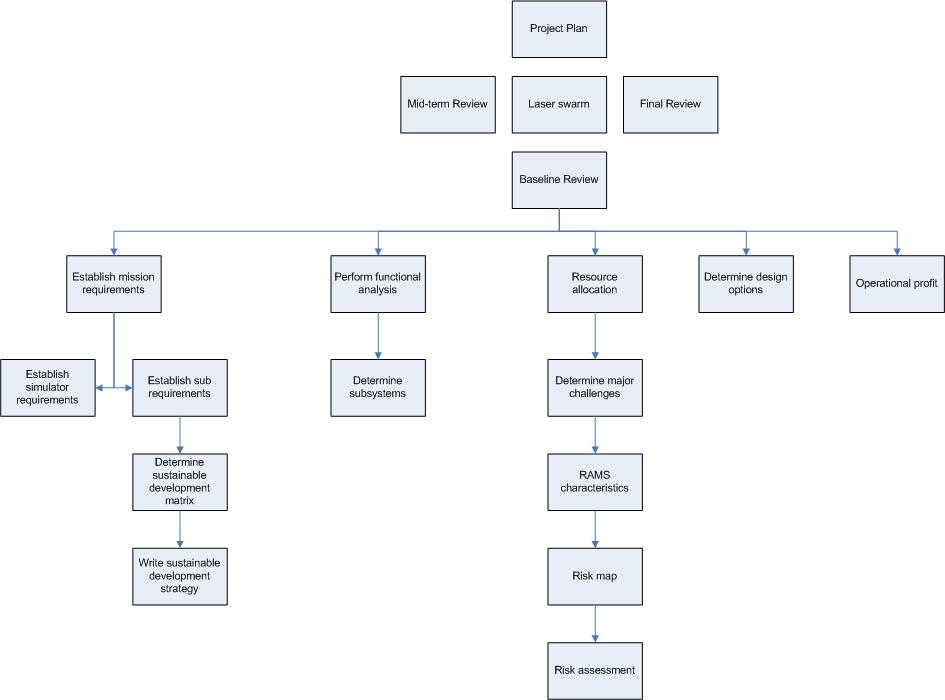
\includegraphics[width=1.0\textwidth, angle=0]{chapters/img/Work_break_down_structure_BR.jpg}
\end{center}
\caption{Work breakdown structure leading to BR.}
\label{wbsbr}
\end{figure}
%\newpage
\begin{figure} [H]
\begin{center}
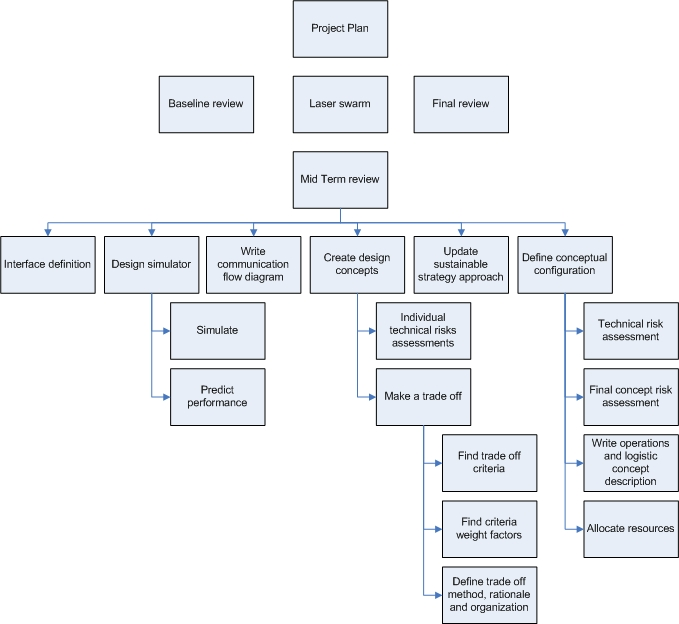
\includegraphics[width=1.0\textwidth, angle=0]{chapters/img/Work_break_down_structure_MTR.jpg}
\end{center}
\caption{Work breakdown structure leading to MTR.}
\label{wbsmtr}
\end{figure}
%\newpage
\begin{figure} [H]
\begin{center}
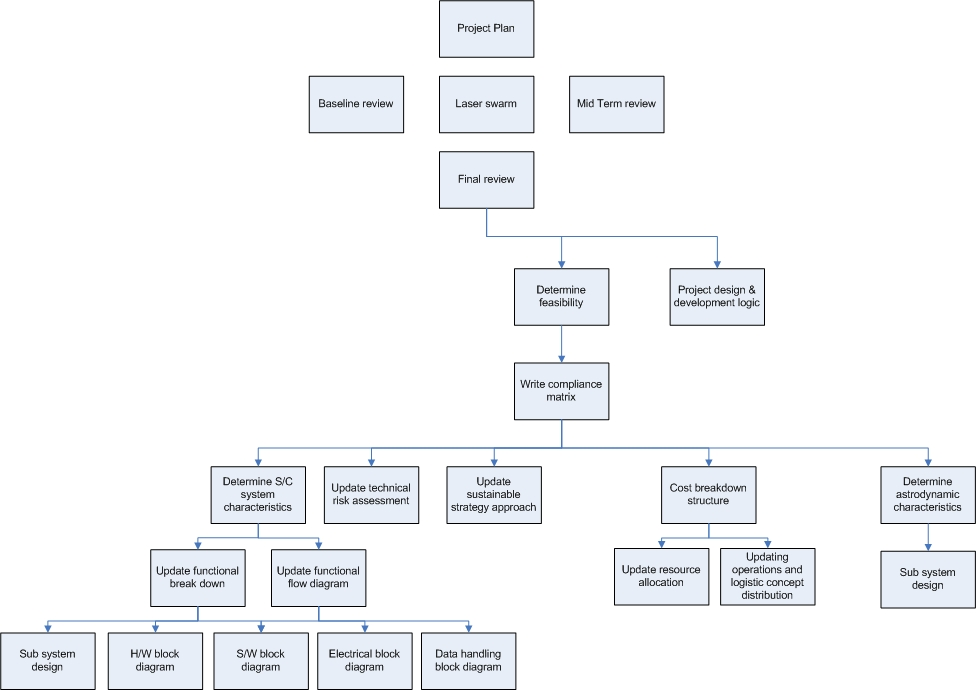
\includegraphics[width=1.0\textwidth, angle=0]{chapters/img/Work_break_down_structure_FR.jpg}
\end{center}
\caption{Work breakdown structure leading to FR.}
\label{wbsfr}
\end{figure}